\documentclass{article}
\usepackage{setspace}
\usepackage{geometry}
\usepackage[utf8]{inputenc}
\usepackage{amsmath,amsthm,amssymb}
\usepackage{mathtools}

\geometry{letterpaper, portrait, margin=1in}
\setstretch{1.5}
\title{Homework 5}
%\date{1-18-2020}
\author{Runmin Lu}

\begin{document}
	\maketitle
	%\newpage
	
	\section*{Exercise 2.8}
	\subsection*{(a)}
		Given any arbitrary $K$ data sets, we can produce $K$ corresponding final hypothesis $g_1, ..., g_K$.\\
		We know that $\forall k \in [1, K]: g_k \in \mathcal H$ and $\mathcal H$ is closed under linear combination.\\
		$\bar g = \frac1K \sum\limits_{k=1}^K g_k$, which is a linear combination of $g_1,...,g_K$. Therefore, $\bar g \in \mathcal H$.
		
	\subsection*{(b)}
		$\mathcal H$ has only 2 function, one that always returns $-1$ and one that always returns $+1$. The learning algorithm picks $g$ randomly. Then $\bar g$ is a function that always returns 0, which is not in $\mathcal H$.
		
	\subsection*{(c)}
		No because depending on the distribution of the data, $\bar g(\mathbf x)$ can take any value between $-1$ and $+1$.
		
	\section*{Problem 2.14}
	\subsection*{(a)}
		Assume $d_{vc}(\mathcal H) \geq K(d_{vc} + 1)$ for contradiction. Then there's a set of $2K(d_{vc} + 1)$ data points that can be shattered by $\mathcal H$. Let's list them all in a table.\\
		\begin{tabular}{|c|c|c|c|c|}
			\hline
			Data Point & 1 & 2 & ... & $K(d_{vc}+1)$\\
			\hline
			Dichotomy 1 & +1 & -1 & ... & +1\\
			\hline
			Dichotomy 2 & +1 & +1 & ... & +1\\
			\hline
			... & ... & ... & ... & ... \\
			\hline
			Dichotomy $2^{K(d_{vc}+1)}$ & -1 & -1& ... & -1\\
			\hline
		\end{tabular}\\\\
		Look at the first $d_{vc}+1$ columns. There must be a dichotomy that can't be implemented by $\mathcal H_1$ because it can't shatter any data set of size $> d_{vc}$. For the same reason, some dichotomy in the second $d_{vc}+1$ can't be implemented by $\mathcal H_2$ and so on. If we concatenate all of them, then it can't be in this table because none of $\mathcal H_1, ..., \mathcal H_K$ implements it, which contradict with that all $2^{K(d_{vc}+1)}$ dichotomies are present. Therefore, $d_{vc}(\mathcal H) < K(d_{vc} + 1)$.
	\subsection*{(b)}
		\begin{align*}
			\text{Assume }d_{vc}(\mathcal H) &> \ell \text{ for contradiction}\\
			\text{Then } m_{\mathcal H}(\ell) &= 2^\ell\\
			\forall i: m_{\mathcal H_i}(\ell) &\leq \ell^{d_{vc}} + 1
		\end{align*}
		Because $\mathcal H$ is the union of all $\mathcal H_i$'s, it can implement at most $\sum\limits_{i=1}^K m_{\mathcal H_i}(\ell)$ dichotomies. Therefore
		\begin{align*}
			m_\mathcal H(\ell) &\leq \sum\limits_{i=1}^K m_{\mathcal H_i}(\ell)\\
			&\leq K(l^{d_{vc}} + 1)
		\end{align*}
		We can assume that $\ell > 0$. If $\ell = 0$, then the premise $2^0 > 2K0^{d_{vc}}$ is always true but then we force $d_{vc}(\mathcal H) = 0$, which isn't always true.\\
		We can also assume that $\ell$ is an integer. Otherwise, as $\lim\limits_{\ell \rightarrow 0^+} 2^\ell = 1 > \lim\limits_{\ell \rightarrow 0^+} 2K\ell^{d_{vc}} = 0$, which is always true but again we force $d_{vc}(\mathcal H) = 0$.\\
		Therefore, for positive integer $\ell$,
		\begin{align*}
			1 &\leq \ell^{d_{vc}}\\
			\ell^{d_{vc}}+1 &\leq 2\ell^{d_{vc}}\\
			m_{\mathcal H}(\ell) &\leq K(l^{d_{vc}} + 1)\\
			&\leq 2K\ell^{d_{vc}}\\
			2^\ell&\leq 2K\ell^{d_{vc}}\\
			\text{Contradiction} \implies d_{vc}(\mathcal H) &\leq \ell
		\end{align*}
	
	\subsection*{(c)}
		\begin{align*}
			\text{Let } \ell &= 7(d_{vc} + K)\log_2(d_{vc}K)\\
			\text{If we can show } 2^\ell &< 2K\ell^{d_{vc}}\\
			\text{Then } d_{vc}(\mathcal H) &\leq \ell = 7(d_{vc} + K)\log_2(d_{vc}K)\\
			\text{Let }d &= d_{vc}\\
			\textbf{LHS } &= 2^{ 7(d+K)\log_2(dK) }\\
			&= (dK)^{7(d+K)}\\
			&= d^{7d}d^{7K}K^{7d}K^{7K}\\
			\textbf{RHS } &= 2K(7(d+K)\log_2(dK))^d\\
			&= 2K(7(d+K)(\log_2d+\log_2K))^d\\
			&< 2K(7(d+K)(d+K))^d\\
			&= 2K(7(d+K)^2)^d\\
		\end{align*}
		Clearly $K^{7K} > 2K$ and $d^{7d}d^{7K}K^{7d} > d^{7d}K^{7d}$ for $K \geq 2$ and $d \geq 1$.\\
		Now we just need to show
		\begin{align*}
			d^{7d}K^{7d} &>(7(d+K)^2)^d\\
			(dK)^7 &> 7(d+K)^2
		\end{align*}
		Base Case: $d = 1, K = 2$\\
		$2^7 = 128 > 7(3^2) = 63$\\
		Inductive Step: $(dK)^7 > 7(d+K)^2 \rightarrow (d(K+1))^7 > 7(d+K+1)^2$
		\begin{align*}
			(d(K+1))^7 &= (dK+d)^7\\
			&= (dK)^7 + d^7(7K^6+21K^5+35K^4+35K^3+21K^2+7K+1)\\
			7(d+K+1)^2 &= 7((d+K)^2+2(d+K)+1)\\
			&= 7(d+K)^2 + 14(d+K) + 7\\
			&= 7(d+K)^2 + 14d+14K + 7
		\end{align*}
		Knowing that $(dK)^7 > 7(d+K)^2$,\\
		it's sufficient to show $d^7(7K^6+21K^5+35K^4+35K^3+21K^2+7K+1) > 14d+14K + 7$ and it's true because clearly
		\begin{align*}
			d^7(7K) &\geq 14 > 7\\
			d^7(21K^2) &> 14K\\
			d^7(35K^3) &> 14d
		\end{align*}
		Therefore $2^\ell < 2K\ell^{d_{vc}} \rightarrow d_{vc}(\mathcal H) \leq 7(d_{vc} + K)\log_2(d_{vc}K)$.\\
		Also combined with the inequality from part (a), $d_{vc}(\mathcal H) \leq \min( K(d_{vc}+1), 7(d_{vc} + K)\log_2(d_{vc}K) )$
	\section*{Problem 2.15}
	\subsection*{(a)}
		$h(x_1, x_2) = sign(x_1 + x_2)$\\
		$+1$ region: everything above the line $x_1 + x_2 = 0$\\
		$-1$ region: everything below the line $x_1 + x_2 = 0$
		
	\subsection*{(b)}
		Lemma: all classifiers with negative slope everywhere and the $+1$ region above the curve are in $\mathcal H$.\\
		Proof by contraposition. Let there be a point $\mathbf x$ and a displacement vector $\Delta \mathbf x \geq \mathbf 0$ and $h$ such that $h(\mathbf x + \Delta \mathbf x) < h(\mathbf x)$. We want to show that $h$ does not satisfy the property in the lemma.\\
		To get from $\mathbf x$ and $\mathbf x + \Delta \mathbf x$, we must cross the curve of $h$. Let the tangent line of that curve have a weight vector $\mathbf w$. Then we have
		\begin{align*}
			\mathbf w^T(\mathbf x + \Delta \mathbf x) &< \mathbf w^T \mathbf x\\
			w_0 + w_1x_1 + w_1\Delta x_1 + w_2x_2 + w_2\Delta x_2 &< w_0 + w_1x_1 + w_2x_2\\
			w_1\Delta x_1 + w_2\Delta x_2 &< 0\\
			\mathbf w^T\Delta \mathbf x &< 0
		\end{align*}
		Because $\Delta \mathbf x$ lies somewhere in the first quadrant, including the axis, and $\mathbf n = (w_1, w_2)$, the normal vector of the tangent line represented by $\mathbf w$, needs to form obtuse angle to $\Delta \mathbf x$, $\mathbf n$ cannot be in the first quadrant. Also because $\mathbf n$ points to the positive region, the tangent line represented by $\mathbf w$ cannot have both negative slope and $+1$ region above. Therefore, all classifiers with negative slopes and the $+1$ region above the curve are in $\mathcal H$.\\
		Now we can construct $N$ arbitrary points that lie in the line $x_1 + x_2 = 0$. $\mathcal H$ shatters them all by going along those points and freely move above or below each point so each point can be assigned $+1$ and $-1$ arbitrarily. Refer to the picture below if the description isn't good enough. Therefore $m_\mathcal H(N) = 2^N$ and $d_{vc} = \infty$.\\
		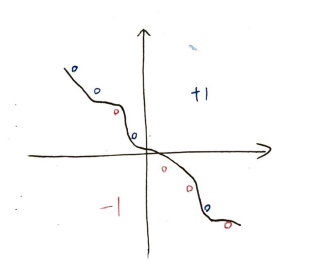
\includegraphics[scale=0.55]{p2.15b.png}
		
	\section*{Problem 2.24}
	\subsection*{(a)}
		Given $\mathcal D$, let the learning algorithm pick $g(x) = ax + b$.
		\begin{align*}
			a &= \frac{x_1^2 - x_2^2}{x_1 - x_2}\\
			&= x_1 + x_2\\
			g(x) &= (x_1 + x_2)(x - x_1) + x_1^2\\
			&= (x_1+x_2)x - x_1x_2\\
			\bar x_1 &= 0\\
			\bar x_2 &= 0\\
			\bar{x_1x_2} &= \frac12\int_{-1}^1\frac12\int_{-1}^1 -x_1x_2 dx_2dx_1\\
			&= 0\\
			\bar g(x) &= \boxed{0}
		\end{align*}
		
	\subsection*{(b)}
		Generate 1000 random data sets. For each of them, compute $g^\mathcal D(x)$ and record the slope and y-intercept. Take the average of all the slopes and all tye y-intercepts to get $\bar g(x)$.\\
		Generate a random test data set of 1000 data points. Loop over it and in an inner loop over all the $g^\mathcal D(x)$'s, compute $(g^\mathcal D(x) - \bar g(x))^2$. Take the average of all of them to get var.\\
		Loop over the same test data set, compute $(f(x) - \bar g(x))^2$. Take the average of all of them to get bias.\\
		Loop over the test data set and in an inner loop over all the $g^\mathcal D(x)$'s, compute $(f(x) - g^\mathcal D(x))^2)$. Take the average to get $E_{\text{out}}$.
		
	\subsection*{(c)}
		$g(x) \approx -0.0103x + 0.0041$\\
		var $\approx 0.3110$\\
		bias $\approx 0.1814$\\
		$E_{\text{out}} \approx 0.4924$\\
		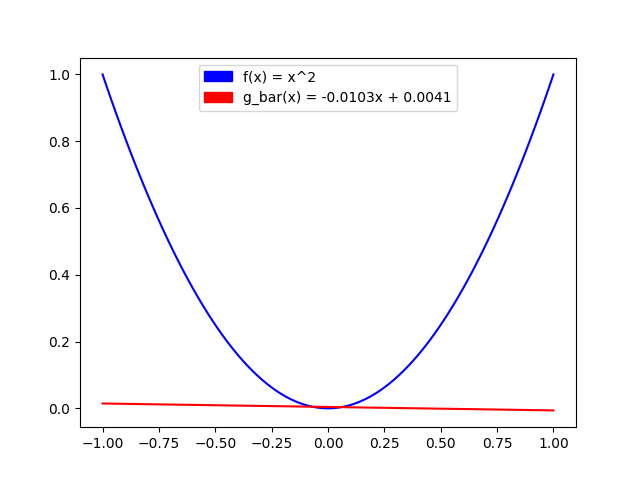
\includegraphics[scale=1]{p2.24c.png}
	
	\subsection*{(d)}
		\begin{align*}
			\text{var} &= E_xE_\mathcal D(g^\mathcal D(x) - \bar g(x))^2\\
			&= \frac12\int_{-1}^1\frac12\int_{-1}^1\frac12\int_{-1}^1((x_1 + x_2)(x - x_1) + x_1^2 - 0)^2 dx_2dx_1dx\\
			&= \boxed{\frac13}\\
			\text{bias} &=  E_xE_\mathcal D(f(x) - \bar g(x))^2\\
			&= \frac12\int_{-1}^1(x^2 - 0)^2 dx\\
			&= \boxed{\frac15}\\
			E_\text{out} &= \text{var} + \text{bias}\\
			&= \frac13 + \frac15\\
			&= \boxed{\frac8{15}}
		\end{align*}
\end{document}